

\chapter{The Natural Numbers}\label{lec:NaturalNumbers}

\begin{goals}
\begin{goal}{Lecture}
\item Present the natural numbers as comprising a structure suited to counting.
\item Identify similar structures that can not properly represent counting.
\item Rule out ``bad'' structures via postulates.
\end{goal}

\begin{goal}{Study}
\item Gain facility in the course's \emph{successor} notation, including
translating between successor notation and base $10$ notation.
\item Commit to memory the postulates of natural numbers.
\item Demonstrate ability to recognize failures of the postulates. 
\end{goal}
\end{goals}

The \emph{natural numbers} have to do with counting: $0$, $1$, $2$, $3$, $\ldots$.
They do not include negatives or fractions or irrationals.
In this lecture, the structure of natural numbers is the topic.
To hone in on that structure, we look at structures similar to the natural numbers, but that fail to capture some basic aspects of counting. 
Bogus structures are ruled out by \emph{postulates} (also known as \emph{axioms}) that distinguish the structure of natural numbers from others.

\section{The Basic Picture}

Our first task is to look back to one of the very first mathematical concepts we all learned, namely, \emph{counting}. Some numbers obviously are meant for conuting. $1$, $2$, $3$, and so on are counting numbers, whereas $-1$, $\frac{1}{2}$ and $\sqrt{2}$  are not. So let's start with a basic intuitive definition: a \emph{counting} or \emph{natural} number is a number that can be used to answer a qeustion of the form ``How many $x$ are there?''
This is distinct, somehow, from ``How \emph{much} $x$?'' The latter sort of question could be answered with $\frac{1}2$ (as long as we know how we are measuring). On the other hand, the answer to a ``how many'' question could be $0$ (``how many professors own unicorns?''). So $0$ shoud be included in our thinking.

Natural numbers are pictured like stepping stones in Figure \ref{fig:nat-numbers}.

\begin{figure}[h]
  \centering
  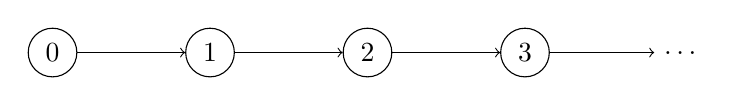
\begin{tikzpicture}
    \node (a) at (0,0) [circle, draw] {0};
    \node (b) at (2,0) [circle,draw] {1}; \node (c) at (4,0)
    [circle,draw] {2}; \node (d) at (6,0) [circle,draw] {3}; \node (e)
    at (8,0) {\ldots}; \draw[->] (a.east) -- (b.west); \draw[->]
    (b.east) -- (c.west); \draw[->] (c.east) -- (d.west); \draw[->]
    (d.east) -- (e.west);
  \end{tikzpicture}
  \caption{A picture of the natural numbers}
  \label{fig:nat-numbers}
\end{figure}


Not all ``stepping stone'' pictures are acceptable.
Figures \ref{fig:NatSigBad1}, \ref{fig:NatSigBad2} and \ref{fig:NatSigBad3} illustrate three ways \emph{not} to picture the natural numbers.

\begin{figure}[h]
\centering
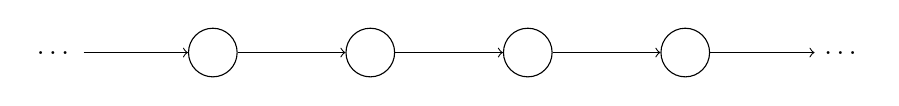
\begin{tikzpicture}
  \node (z) at (-2,0) {\ldots}; 
\node (a) at (0,0) [circle, draw] {\phantom0};
    \node (b) at (2,0) [circle,draw] {\phantom0}; \node (c) at (4,0)
    [circle,draw] {\phantom0}; \node (d) at (6,0) [circle,draw] {\phantom0}; 
    \node (e) at (8,0) {\ldots}; 
    \draw[->] (z.east) -- (a.west); \draw[->] (a.east) -- (b.west); \draw[->]
    (b.east) -- (c.west); \draw[->] (c.east) -- (d.west); \draw[->]
    (d.east) -- (e.west);
%\node (left) at (0,0) [circle,draw] {}; \node (center) at (1,0)
%  [circle,draw] {}; \node (right) at (2,0) [circle,draw] {}; \draw[<-]
%  (left.north east)--(center.north west); \draw[->] (center.south
%  east)--(right.south west); \draw[->] (left.south
%  east)--(center.south west); \draw[<-] (center.north
%  east)--(right.north west);
\end{tikzpicture}
\caption{Nowhere to start}\label{fig:NatSigBad1}

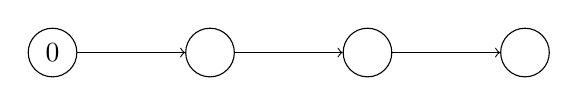
\begin{tikzpicture}
  \node (a) at (1,0) [circle, draw] {0};
    \node (b) at (3,0) [circle,draw] {\phantom0}; \node (c) at (5,0)
    [circle,draw] {\phantom0}; \node (d) at (7,0) [circle,draw] {\phantom0}; 
    \draw[->] (a.east) -- (b.west); \draw[->]
    (b.east) -- (c.west); \draw[->] (c.east) -- (d.west);
\end{tikzpicture}
\caption{Nowhere to go}\label{fig:NatSigBad2}

\begin{tikzpicture}
%    \node (a) at (0,0) [circle, draw] {0};
    \node (b) at (2,0) [circle,draw] {0}; 
    \node (c) at (4,0) [circle,draw] {\phantom0}; 
    \node (d1) at (6,1) [circle,draw] {\phantom0}; 
    \node (d2) at (6,-1) [circle,draw] {\phantom0}; 
    \node (e1) at (8,1) [circle,draw] {\phantom0}; 
    \node (e2) at (8,-1) [circle,draw] {\phantom0};
    \node (f) at (10,0) [circle,draw] {\phantom0};
    \node (g) at (12,0) {\ldots};
%    \draw[->] (a.east) -- (b.west); 
    \draw[->] (b.east) -- (c.west); 
\draw[->] (c.north east) -- (d1.west);
\draw[->] (c.south east) -- (d2.west);
\draw[->] (d1.east) -- (e1.west);
\draw[->] (d2.east) -- (e2.west);
\draw[->] (e1.south east) -- (f.west);
\draw[->] (e2.north east) -- (f.west);
\draw[->] (f.east) -- (g.west);
\end{tikzpicture}
\caption{Forks in the path}\label{fig:NatSigBad3}
\end{figure}

These incorrect pictures can be ruled out by explaining the basic structure of counting. We will ``explain the obvious'' by stating things like this as \emph{postulates}.

%\refstepcounter{axiomCnt}
\begin{postulate}[Basic Structure of Natural Numbers]\label{post:NatSig}
The \newterm{natural numbers} have the following basic structure.
  \begin{itemize}
  \item There is a special natural number. We denote this by $0$.
  \item For any natural number $n$, there is
    a unique \emph{next} natural number. We call this the \newterm{successor of $n$}. 
    In these lectures, we denote the successor of $n$ by $n^\nxt$.
  \end{itemize}
\end{postulate}

According to Postulate \ref{post:NatSig}, $0$, $0^\nxt$, $0^{\nxt\nxt}$, $0^{\nxt\nxt\nxt}$ each denote a natural number. 
Of course, we usually abbreviate them by writing $0$, $1$, $2$, $3$.
But the \emph{characters} $1$, $2$, $3$, etc., are not related to each other in any way.
The notation we are using here makes it completely clear that $0^\nxt$ is the number after $0$, and so on. 
We will want to be able to switch between the familiar ``decimal' notation and ``successor'' notation whenever it is convenient.

\begin{exer}
\begin{multicols}{2}
%\begin{itemize}
\item Convert the following from decimal notation to successor notation.
  \begin{exercise}
  \item $9$
  \item $10$
  \item $4 + 3$
  \item $n + 4$
  \end{exercise}
\item Convert the following to from successor notation to decimal notation.
\begin{exercise}
\item $0^{\nxt\nxt\nxt\nxt}$
\item $n^{\nxt\nxt\nxt\nxt\nxt}$
\item $5^{\nxt\nxt}$
\item $0^\nxt + 0^{\nxt\nxt}$
\end{exercise}
%\end{itemize}
\end{multicols}
\end{exer}

\printbreak

\section{Narrowing the possibilities}

Figures \ref{fig:one-loop} and \ref{fig:two-loop} illustrate 
problems that Postulate \ref{post:NatSig} does not avoid.

\begin{figure}[ht]
  \centering
  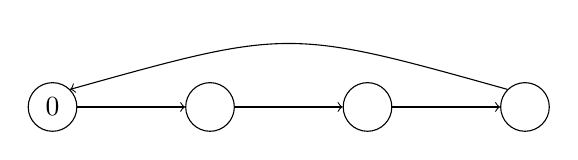
\begin{tikzpicture}
    \node (a) at (0,0) [circle, draw] {$0$}; \node (b) at (2,0)
    [circle,draw] {\phantom{$0$}}; \node (c) at (4,0) [circle,draw]
    {\phantom{$0$}}; \node (d) at (6,0) [circle,draw] {\phantom{$0$}};
    \draw[->] (a.east) -- (b.west); \draw[->] (b.east) -- (c.west);
    \draw[->] (c.east) -- (d.west); \draw[->] (d.north west)
    .. controls (3,1) .. (a.north east);
  \end{tikzpicture}
  \caption{A strange way to count}
  \label{fig:one-loop}
\end{figure}

\begin{figure}[ht]
  \centering
  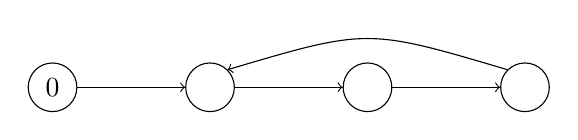
\begin{tikzpicture}
    \node (a) at (0,0) [circle, draw] {$0$}; \node (b) at (2,0)
    [circle,draw] {\phantom{$0$}}; \node (c) at (4,0) [circle,draw]
    {\phantom{$0$}}; \node (d) at (6,0) [circle,draw] {\phantom{$0$}};
    \draw[->] (a.east) -- (b.west); \draw[->] (b.east) -- (c.west);
    \draw[->] (c.east) -- (d.west); \draw[->] (d.north west)
    .. controls (4,.75) .. (b.north east);
  \end{tikzpicture}
  \caption{Another strange way to count}
  \label{fig:two-loop}
\end{figure}
\clearpage

\begin{exer}
\begin{exercise}
\item Explain, in one or two sentences each, why Figures \ref{fig:one-loop} and \ref{fig:two-loop} depict systems that agree with Postulate \ref{post:NatSig}.
\end{exercise}
\end{exer}
\ipadbreak

Figure \ref{fig:one-loop} is flawed because $0$ has a
\emph{predecessor}: a value $n$ satisfying $0^{\nxt\nxt\nxt\nxt} = 0$. Figure
\ref{fig:two-loop} is flawed because an element has two distinct
predecessors: $0^\nxt = 0^{\nxt\nxt\nxt\nxt}$.  We can insist that
these flaws do not happen in the natural numbers. That is, 
we rule them out with axioms.

\begin{postulate}{Nothing Precedes $0$}\label{post:NatZero}
  For every natural number $n$, $n^\nxt\neq 0$.
\end{postulate}

\begin{postulate}{Predecessors are Unique}\label{post:NatPred}
  For any natural numbers $m$ and $n$, if $m^\nxt=n^\nxt$ then $m=n$.
\end{postulate}

These postulates eliminate Figures \ref{fig:one-loop}, \ref{fig:two-loop} and similar pictures.  
But there is still a subtle problem. 
Consider Figure \ref{fig:nonstandard}.

\begin{figure}[h]
  \centering
  \begin{tikzpicture}
    \node (a) at (0,0) [circle, draw] {$0$}; \node (b) at (2,0)
    [circle,draw] {\phantom{$0$}}; \node (c) at (4,0) [circle,draw]
    {\phantom{$0$}}; \node (d) at (6,0) [circle,draw] {\phantom{$0$}};
    \node (e) at (8,0) {\ldots}; \draw[->] (a.east) -- (b.west);
    \draw[->] (b.east) -- (c.west); 
    \draw[->] (c.east) -- (d.west);
    \draw[->] (d.east) -- (e.west);
    % \node (z) at (0,2) {\ldots};
    \node (aa) at (2,2) [circle, draw] {$\star$}; \draw[->] (aa.east)
    .. controls (3.5,3) and (0.5,3) .. (aa.west);
    % \node (bb) at (4,2) [circle,draw] {\phantom{$0$}}; \node (cc) at
    % (6,2) [circle,draw] {\phantom{$0$}}; \node (dd) at (8,2)
    % [circle,draw] {\phantom{$0$}}; \node (ee) at (10,2) {\ldots};
    % \draw[->] (z.east) -- (aa.west); \draw[->] (aa.east) --
    % (bb.west); \draw[->] (bb.east) -- (cc.west); \draw[->] (cc.east)
    % -- (dd.west); \draw[->] (dd.east) -- (ee.west);
  \end{tikzpicture}
  \caption{A model of the natural numbers?}
  \label{fig:nonstandard}
\end{figure}

This picture satisfies the first three postulates. 
Yet, it is not a picture of natural numbers because it has ``extra stuff'' in it ($\star$).

\ipadbreak

To rule out ``extra stuff'', we formulate our final postulate for natural numbers.
We diagnose the problem as follows.
Were we to erase the circle labelled $\star$ and any the arrows leading to and from it, the remaining part of Figure \ref{fig:nonstandard} would still live up to Postulate \ref{post:NatSig}.
This is exactly what we mean by ``extra stuff'': 
elements that can be removed without violating the Postulate \ref{post:NatSig} (the essential structure). 
This leads to our last axiom. 

\begin{postulate}{The Axiom of Induction}\label{post:NatInd}
 No natural numbers can be removed without violating \ref{post:NatSig}.
\end{postulate}

%Believe it or not, the four axioms we have stated here completely
%characterize the standard picture of the natural numbers. In other
%words, any picture that satisfies these axioms will look the same. A
%rigorous proof of this is possible, but not necessary for now.

\begin{exer}
\begin{exercise}
\item Each of the following pictures fails to satisfy either the one or more of our axioms. 
For each, explain which axioms are violated.
\begin{multicols}{2}
\begin{enumerate}
\item
  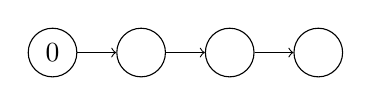
\begin{tikzpicture}[scale=.75]
    \node (a) at (0,0) [circle, draw] {$0$}; \node (b) at (1.5,0)
    [circle,draw] {\phantom{$0$}}; \node (c) at (3,0) [circle,draw]
    {\phantom{$0$}}; \node (d) at (4.5,0) [circle,draw] {\phantom{$0$}};
    \draw[->] (a.east) -- (b.west); \draw[->] (b.east) -- (c.west);
    \draw[->] (c.east) -- (d.west);
  \end{tikzpicture}
\item
  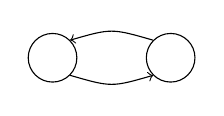
\begin{tikzpicture}[scale=.75]
    \node (a) at (0,0) [circle, draw] {\phantom{$0$}};
    \node (b) at (2,0) [circle, draw] {\phantom{$0$}};
    \draw[->] (a.south east) .. controls (1,-.5) .. (b.south west);
    \draw[->] (b.north west) .. controls (1,.5) .. (a.north east);
  \end{tikzpicture}
\item  
  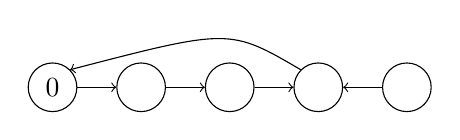
\begin{tikzpicture}[scale=.75]
    \node (a) at (0,0) [circle, draw] {$0$}; \node (b) at (1.5,0)
    [circle,draw] {\phantom{$0$}}; \node (c) at (3,0) [circle,draw]
    {\phantom{$0$}}; \node (d) at (4.5,0) [circle,draw] {\phantom{$0$}};
    \node (e) at (6,0) [circle,draw] {\phantom{$0$}};
    \draw[->] (a.east) -- (b.west); \draw[->] (b.east) -- (c.west);
    \draw[->] (c.east) -- (d.west); \draw[->] (d.north west)
    .. controls (3,1) .. (a.north east);
    \draw[->] (e.west) -- (d.east);
  \end{tikzpicture}
\item
  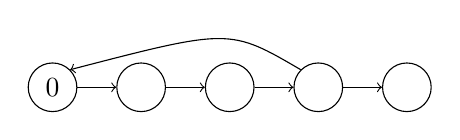
\begin{tikzpicture}[scale=.75]
    \node (a) at (0,0) [circle, draw] {$0$}; \node (b) at (1.5,0)
    [circle,draw] {\phantom{$0$}}; \node (c) at (3,0) [circle,draw]
    {\phantom{$0$}}; \node (d) at (4.5,0) [circle,draw] {\phantom{$0$}};
    \node (e) at (6,0) [circle,draw] {\phantom{$0$}};
    \draw[->] (a.east) -- (b.west); \draw[->] (b.east) -- (c.west);
    \draw[->] (c.east) -- (d.west); \draw[->] (d.north west)
    .. controls (3,1) .. (a.north east);
    \draw[->] (d.east) -- (e.west);    
  \end{tikzpicture}
\end{enumerate}
\end{multicols}

\item\label{exer:cases} I have in mind a picture for the Basic Vocabulary \ref{post:NatSig} and that satisfies Axioms \ref{post:NatZero}
and \ref{post:NatPred}. Furthermore, in that picture, I have in mind and element $n$ for which (a) $n\neq 0$
and (b) $n$ has no predecessor (that is, $n\neq m^\nxt$ for every $m$). Convince me that
the picture fails to satisfy Axiom \ref{post:NatInd}.
\item\label{exer:CyclicModel} Draw three different pictures of situations that satisfies all the postulates except that they fail Postulate \ref{post:NatZero}. So there will be an arrow from a bubble into the bubble $0$. The result must satisfy all other postulates including the Axiom of Induction.
\end{exercise}
\end{exer}

The latest exercise shows that in the natural numbers, if $n\neq 0$, then $n = m^\nxt$ for some $m$. In other
words, every non-zero natural number has a predecessor. 


\chapter{Arithmetic}\label{lec:Arithmetic}


\begin{goals}
\tightlists
\noindent\textbf{Lecture}
\begin{itemize}
\item Present addition and multiplication via defining equations.
\item Practice using the defining equations to calculate sums and products.
\end{itemize}

\noindent\textbf{Study}
\begin{itemize}
  \item Understand addition and multiplication as characterized by defining equations.
  \item Be able to explain how addition and multiplication relate to counting.
  \item Exhibit competence in calculating sums and products from the defining equations.
\end{itemize}
\defaultlists
\end{goals}

Adding and multiplying arise from counting. In this section, we explore how to define them purely in terms of counting.

\ipadbreak
\printbreak

\section{Basic Arithmetic Operations}

We know that addition ``works'' by counting ahead. For example, to \emph{add} $4+5$, we can start with $4$ and then count up five more. Likewise, multiplication ``works'' by counting a number of additions. For example, to multiply $2\cdot 3$ we can add $2$ three times: $2+2+2$. The following definitions capture the idea.
 
\begin{defn}[Arithmetic Operations]\label{def:NatArithmetic}
\noindent The \newterm{sum} of two natural numbers, $m$ and $n$, is a natural number (denoted by $m+n$). For every natural number $m$, the following 
are true:
\begin{align*}
    m + 0     &= m\\
    m + k^\nxt &= (m + k)^\nxt &&\text{for any natural number $k$}
\end{align*}

\noindent The \newterm{product} of two natural numbers, $m$ and $n$, is a natural number 
(denoted by $m\cdot n$). For every natural number $m$, the following are true:
\begin{align*}
  m\cdot 0 &= 0\\
  m\cdot k^\nxt &= m + (m\cdot k) &&\text{for any natural number $k$}
\end{align*}
\end{defn}


A moment's thought about arithmetic should convince you that these equations are reasonable.
Certainly $m+0=m$ and $m\cdot 0 = 0$ should be true for any $m$. 
The second equation for $+$ can be read as saying ``to add $m$ to the successor of $k$, simply add $m$ to $k$, then take the successor.''
The second equation for $\cdot$ can be read as saying ``to multiply $m$ by the successor of $k$, simply multiply $m$ by $k$, and add $m$ to the result.''

The Axiom of Induction ensures that there are indeed unique operations $+$ and $\cdot$ that satisfy the equations.
A proof of this fact is not particularly illuminating right now, so let us agree to take it for granted.

\begin{example}
Do the defining equations for addition really explain how to add? Let's use them to calculate
$4+3$:
\begin{align*}
  4 + 3 &= 4 + 0^{\nxt\nxt\nxt}&&\text{[$3$ abbreviates $0^{\nxt\nxt\nxt}$]}\\
  &= 4^\nxt + 0^{\nxt\nxt} &&\text{[$m + k^\nxt = m^\nxt+k$]}\\
  &= 4^{\nxt\nxt} + 0^\nxt &&\text{[Same reason]}\\
  &= 4^{\nxt\nxt\nxt} + 0 &&\text{[Same reason]}\\
  &= 4^{\nxt\nxt\nxt} &&\text{[$m+0 = m$]}\\
  &= (0^{\nxt\nxt\nxt\nxt})^{\nxt\nxt\nxt} && \text{[$4$ abbreviates $0^{\nxt\nxt\nxt\nxt}$]}\\
  &= 0^{\nxt\nxt\nxt\nxt\nxt\nxt\nxt} && \text{[Remove unneeded parentheses]}\\
  &= 7 &&\text{[$7$ abbreviates $0^{\nxt\nxt\nxt\nxt\nxt\nxt\nxt}$]}
\end{align*}
\end{example}
\ipadbreak

\begin{example}
A product can be calculated similarly. Consider $2\cdot 2$.
\begin{align*}
  2\cdot 2 &= 2\cdot 0^{\nxt\nxt} &&\text{[$2$ abbreviates $0^{\nxt\nxt}$]}\\
           &= 2 + (2\cdot 0^\nxt) &&\text{[$m\cdot k^\nxt = m + (m\cdot k)$]}\\
           &= 2 + (2 + (2\cdot 0))&&\text{[Same reason]}\\
           &= 2 + (2 + 0) &&\text{[$m\cdot 0=0$]}\\
           &= 2 + 2&&\text{[$m+0 = m$]}\\
           &= 2 + 0^{\nxt\nxt}&&\text{[$2$ abbreviates $0^{\nxt\nxt}$]}\\
           &= 2^\nxt + 0^\nxt &&\text{[$m+k^\nxt = m^\nxt+k$]}\\
           &= 2^{\nxt\nxt} + 0&&\text{[Same reason]}\\
           &= 2^{\nxt\nxt} &&\text{[$m+0 = m$]}\\
           &= (0^{\nxt\nxt})^{\nxt\nxt} &&\text{[$2$ abbreviates $0^{\nxt\nxt}$]}\\
           &= 0^{\nxt\nxt\nxt\nxt}&&\text{[Remove unnecessary parentheses]}\\
           &= 4 &&\text{[$4$ abbreviates $0^{\nxt\nxt\nxt\nxt}$]}
\end{align*}
\end{example}

We certainly will not want to calculate this way in real life. 
After all, it took twelve steps just to figure $2\cdot 2=4$. But these
examples and the following exercises show how addition and multiplication are
closely tied to simple counting. 

\ipadbreak

\begin{exer}
\begin{exercise}
\item Calculate these sums, following the previous example to write
  each step of your calculation explicitly. Include the reason for
  each step (as in the previous example).Take care to lay out the
  chain of equalities correctly, and do not skip any steps.
\begin{enumerate}
\item $2+4$
\item $4+2$
\item $3+(3+1)$
\item $(3+3)+1$
\item $0 + 3$
\end{enumerate}

\item Notice that it takes more steps to calculate $2+4$ than $4+2$, even though we know they will produce the same answer. Explain why.

\item Calculate the following values, writing each step explicity. 
 \begin{enumerate}
    \item $2\cdot 3$
    \item $0\cdot 2$
    \item $2\cdot(2\cdot 2)$
    \item $3\cdot(2 + 1)$
    \item $(3\cdot 2) + (3\cdot 1)$
    \end{enumerate}
\item Write a definition of exponentiation via defining equations. Follow the pattern
of definition I have written for addition and multiplication.
\end{exercise}
\end{exer}

\chapter{Laws of Arithmetic}\label{lec:ArithmeticLaws}

\begin{goals}
\noindent\textbf{Lecture}
\begin{itemize}
\item Present the most common Laws of Arithmetic for natural numbers.
\item Explain the method of \emph{proof by simple induction}
\item Prove a representative sample of the laws by simple induction.
\end{itemize}
\noindent\textbf{Study}
\begin{itemize}
\item Become familiar with the common names for the Laws of Arithmetic.
\item Pay particular attention to the Laws of Positivity and Cancellativity (they may be the least familiar to you).
\item Demonstrate the ability to identify the main parts of a proof by simple induction.
\item Demonstrate the ability to construct the parts of a proof by simple induction.
\item Prove the remaining laws for yourself.
\end{itemize}
\end{goals}

Before working the last exercises, you knew that $3\cdot (2+1)$ and $3\cdot 2+ 3\cdot 1$
would come out the same because of a law of arithmetic known as \emph{distributivity}. 
Addition and multiplication satisfy several other laws.

\ipadbreak
\printbreak

%\section{Basic Laws}

The following list summarizes several useful laws of
arithmetic on the natural numbers. They are organized to emphasize
similarities between addition and multiplication.

\begin{laws}
\noindent For any natural numbers, $m$, $n$ and $p$:

\begin{tabular}{lr@{\,}l@{\qquad}lr@{\,}l}
\textbf{Associativity}& $m + (n + p)$      &$= (m+n)+p$           &\textbf{Commutativity}&$m + n$    &$= n + m$\\
                      &$m \cdot(n\cdot p)$ &$= (m\cdot n)\cdot p$ &                      &$m\cdot n$ &$= n\cdot m$\\
&&&&&\\ 
\textbf{Identity}&$m + 0$    &$= m$&\textbf{Positivity}&\multicolumn{2}{c}{if $m + n = 0$ then $m=0$}\\
                 &$m\cdot 1$ &$= m$&                   &\multicolumn{2}{c}{if $m\cdot n = 1$ then $m=1$}\\
&&&&&\\
\textbf{Cancellativity}&\multicolumn{2}{c}{if $m + p = n+p$ then $m=n$}&&&\\
                       &\multicolumn{2}{c}{if $m \cdot p^\nxt = n\cdot p^\nxt$ then $m=n$}&&&\\
&&&&&\\
\textbf{Distributivity}&$m\cdot(n+p)$&$= (m\cdot n) + (m\cdot p)$&&&\\
&&&&&\\
\textbf{Case Distinction}&\multicolumn{2}{c}{if $m\neq 0$ then $m=k^\nxt$ for some $k$}&&&\\
\end{tabular}
\end{laws}
\medskip

Most of these laws are familiar and are listed with their common names. The Law of Case
Distinction was the subject of Lecture \ref{lec:NatNumbers} Exercise \ref{exer:cases}. \emph{Go back and look at that exercise again}.
The Law of Positivity for multiplication is not a common name, but
I have used it to emphasize the analogies between addition and multiplication.
Also Case Distinction does not really have a common name. I made that up.

\ipadbreak

\section{Inductive Proofs}

Suppose we wish to prove that every natural number has some
property. For example, let us suppose we wish to prove that every
natural number is \emph{mimsy}.  I have no idea what a mimsy number
is, but let us try to prove this anyway. We could try proving that $0$
is mimsy, $1$ is mimsy, $2$ is mimsy, and so on.  But this won't work
because our proof will never end. In fact, it is not so obvious that
we, humans with finite minds, can ever prove that some property is
true for \emph{all} natural numbers, since it seems to involve
checking infinitely many individual cases.

The Axiom of Induction provides a way forward in spite of our
limitations.  Suppose we were to show that the mimsy natural numbers
all by themselves constitute a picture of Signature
\ref{post:NatSig}.  Then there could not be any natural numbers
left out, for otherwise, we could erase all the non-mimsy natural
numbers and still have a picture of \ref{post:NatSig}. This
is exactly what the Axiom of Induction forbids: we can not erase
\emph{anything} without breaking the signature.

So to prove that all natural numbers are mimsy, we simply need to
prove that
\begin{itemize}
\item $0$ is mimsy, and
\item for all natural numbers $k$, if $k$ is mimsy so is $k^\nxt$.
\end{itemize}
From these, we conclude that the mimsy natural numbers by themselves form a picture of \ref{post:NatSig}. So the Axiom of Induction ensures that all natural numbers
are mimsy.

%\begin{usage}
%  A proof employing the Axiom of Induction in this way is called a
%  proof \emph{by simple arithmetic induction}, or just a proof \emph{by
%    induction}, for short.  We will see more general forms of
%  induction later.
%\end{usage}

To make inductive proofs easier to understand, we often write them
using a three step outline, as illustrated here.
\begin{itemize}
\item{}[Basis] Prove that $0$ is mimsy.
\item{}[Inductive Hypothesis] Assume that $k$ is mimsy.
\item{}[Inductive Step] Prove that $k^\nxt$ is mimsy. [You may use the
  assumption that $k$ is mimsy in this part of the proof.]
\end{itemize}

More practical examples are next.

\begin{prop}

  \emph{Addition is associative.}

\begin{proof}
  We need to show that $m + (n+p) = (m+n)+p$ for all $m$, $n$ and $p$.
  Let us suppose that $m$ and $n$ are fixed values (not known to us).
  We now prove that the values $p$ for which $m+(n+p) = (m+n)+p$ holds
  form a picture of \ref{post:NatSig}.
  \begin{itemize}
  \item{}[Basis] $m+(n+0) = m+n = (m+n)+0$. Both steps are due to the
    defining equations of $+$.
  \item{}[Inductive Hypothesis] Assume $m+(n+k) = (m+n)+k$.
  \item{}[Inductive Step] We must show that $m+(n+k^\nxt) =
    (m+n)+k^\nxt$. 
    \begin{align*}
      m+(n+k^\nxt) &= m + (n+k)^\nxt &&\text{[Def. of +]}\\
      &= (m+(n+k))^\nxt&&\text{[Same]}\\
      &= ((m+n)+k)^\nxt&&\text{[Inductive Hypothesis]}\\
      &= (m+n)+k^\nxt &&\text{[Def. of $+$]}
    \end{align*}
  \end{itemize}
  Therefore (by the Axiom of Induction), $m+(n+p) = (m+n)+p$ holds for
  all $p$. Since the argument does not depend on any extra assumptions
  about $m$ and $n$, it holds for all $m$ and $n$.
\end{proof}
\end{prop}

\printbreak

In the remainder of this section, we further illustrate the technique of simple arithmetic induction via proofs of other laws of arithmetic.

\ipadbreak

\begin{prop}\label{prop:AddZero}
  $0$ is the identity for addition.

\begin{proof}
  We must prove that $m+0 = m = 0 + m$ for all $m$. The first equality is true by the definition of $+$.
  But the second equality, $m = 0 + m$, is not explicitly one of the defining facts about $+$. So we proceed by induction on $m$.
  \begin{itemize}
  \item{}[Basis] $0+0 = 0$ is true by definition of $+$.
  \item{}[Inductive Hypothesis] Assume $0 + k = k$.
  \item{}[Inductive Step] We must show that $0 + k^\nxt = k^\nxt$.
    \begin{align*}
      0 + k^\nxt &= (0+k)^\nxt &&\text{[Def. of $+$]}\\
      &= k^\nxt &&\text{[Inductive hypothesis]}
    \end{align*}
  \end{itemize}
  Therefore, $0+m=m$ holds for all $m$.
\end{proof}
\end{prop}

\ipadbreak

To prove that addition is commutative, we need an additional fact
about how successor and addition interact. 
Mathematicians use the word \emph{lemma} to indicate that a certain fact is only needed to make others proofs easier and is not necessarily valuable in its own right.

\printbreak

\begin{lem}\label{lem:AddSucc}
  For any $m$ and $n$, $(m + n)^\nxt = m^\nxt + n$.

 \begin{proof}
   By induction on $n$:
   \begin{itemize}
   \item{}[Basis]
     \begin{align*}
       (m + 0)^\nxt &= m^\nxt     &&\text{[Def. of $+$]}\\
       &= m^\nxt + 0 &&\text{[Def. of $+$]}
     \end{align*}
   \item{}[Inductive Hypothesis]
    Assume $(m + k)^\nxt = m^\nxt + k$ for some $k$.
   \item{}[Inductive Step]
    We must show that $(m + k^\nxt)^\nxt = m^\nxt + k^\nxt$.
    \begin{align*}
      (m + k^\nxt)^\nxt &= ((m + k)^\nxt)^\nxt && \text{[Def. of $+$]}\\
                     &= (m^\nxt + k)^\nxt &&\text{[Inductive Hypothesis]}\\
                     &= m^\nxt + k^\nxt   &&\text{[Def. of $+$]}
    \end{align*}
   \end{itemize}
So $(m + n)^\nxt = m^\nxt + n$. Because the proof does not depend on any assumption about $m$, it is valid
for all $m$.
 \end{proof}
\end{lem}

Roughly speaking this lemma permits us to move $\nxt$ anywhere within an addition: $m^\nxt + n = (m+n)^\nxt = m+n^\nxt$. So we are free to move a successor ``out of the way'' whenever we need to. The next proof illustrates the point.

\printbreak

\begin{prop}

  \emph{Addition is commutative.}

\begin{proof}
  We need to show that $m+n = n + m$ for all $m$ and $n$.  This time,
  the proof is by induction on $m$. Fix a value for $n$.
  \begin{itemize}
  \item{}[Basis] $0 + n = n = n + 0$ holds because of Proposition
    \ref{prop:AddZero} and the definition of $+$.
  \item{}[Inductive Hypothesis] Assume that $k + n = n + k$ for some
    $k$.
  \item{}[Inductive Step] We must show that $k^\nxt + n = n + k^\nxt$.
    \begin{align*}
      k^\nxt + n &= (k + n)^\nxt&&\text{[Lemma \ref{lem:AddSucc}]}\\
      &=  (n+k)^\nxt&&\text{[Inductive Hypothesis]}\\
      &= n + k^\nxt&&\text{[Def. of $+$]}
    \end{align*}
  \end{itemize}
  Therefore, $m + n = n + m$ for all $m$. Since this argument does not
  depend on any assumptions about $n$, it is valid for all $n$.
\end{proof}
\end{prop}

The next law may be less familiar to you. Roughly, it says that we can ``subtract'' equals and get equals. But note that actual subtraction does not always make sense for natural numbers. We can not, for example, say what $5-7$ means without introducing negative numbers.

\printbreak

\begin{prop}
  \emph{Addition is cancellative.}

\begin{proof}
  We need to prove that if $m + p= n+p$, then $m=n$.  This proof is a little subtler than the previous ones. But notice that is
  still follows the same form.
  
  The proof is by induction on $p$. Assume that $m$ and $n$ are some fixed natural numbers.
  \begin{itemize}
  \item{}[Basis] Suppose $m+0 = n+ 0$. Then immediately by definition
    of $+$, $m=n$.
  \item{}[Inductive Hypothesis] Assume that the following statement is true for some $k$: if $m + k = n + k$ then $m=n$.
  \item{}[Inductive Step] We must show that 
    if $m+k^\nxt = n+k^\nxt$ then $m=n$. Suppose $m+k^\nxt = n + k^\nxt$ [call this (*) for reference]. Then
    \begin{align*}
      (m+k)^\nxt & = m + k^\nxt &&\text{[Def. of $+$]}\\
      & = n + k^\nxt &&\text{[By the supposition (*)]}\\
      & = (n+k)^\nxt &&\text{[Definition of $+$]}
    \end{align*}
    Hence, by Axiom \ref{ax:NatPred} $m+k=n+k$. So by the Inductive Hypothesis, $m=n$.
  \end{itemize}
  Therefore, $m + p = n + p$ implies $m = n$ for all $p$. Since this argument does not
depend on any assumptions regarding $m$ and $n$, it is valid for all $m$ and $n$.
\end{proof}
\end{prop}
\ipadbreak

To prove that multiplication is commutative and cancellative, we will
need the following technical facts (analogous to Proposition
\ref{prop:AddZero} and Lemma \ref{lem:AddSucc}).

\begin{lem}\label{lem:MultZero}
  For any $n$, $0\cdot n = 0$

  \begin{proof}
    The proof is by induction on $n$.
    \begin{itemize}
    \item{}[Basis] $0\cdot 0 = 0$ by definition of $\cdot$.
    \item{}[Inductive Hypothesis] Assume that $0\cdot k = 0$ for some
      $k$.
    \item{}[Inductive Step] We must show that $0\cdot k^\nxt = 0$.
      \begin{align*}
        0\cdot k^\nxt &= 0 + 0\cdot k &&\text{[Definition of $\cdot$]}\\
        &= 0 + 0 &&\text{[Inductive Hypothesis]}\\
        &= 0&&\text{[Definition of $+$]}
      \end{align*}
    \end{itemize}
  \end{proof}
\end{lem}

\ipadbreak

\begin{lem}\label{lem:MultSucc}
  For any $m$ and $n$, $m^\nxt \cdot n = m\cdot n + n$

 \begin{proof}
   The proof is by induction on $n$.
   \begin{itemize}
   \item{}[Basis] $m^\nxt\cdot 0 = 0 = 0+0 = m\cdot 0 + 0$ all follow
     from the definitions of $+$ and $\cdot$.
   \item{}[Inductive Hypothesis] Assume that $m^\nxt\cdot k = m\cdot k +
     k$ for some $k$.
   \item{}[Inductive Step] We must show that $m^\nxt\cdot k^\nxt =
     m\cdot k^\nxt + k^\nxt$.
     \begin{align*}
       m^\nxt\cdot k^\nxt &= m^\nxt + m^\nxt\cdot k &&\text{[Exercise]}\\
       &= (m + m^\nxt\cdot k)^\nxt &&\text{[Exercise]}\\
       &= (m + (m\cdot k + k))^\nxt && \text{[Exercise]}\\
       &= ((m+ m\cdot k) + k)^\nxt &&\text{[Exercise]}\\
       &= (m\cdot k^\nxt + k)^\nxt &&\text{[Exercise]}\\
       &= m\cdot k^\nxt + k^\nxt &&\text{[Exercise]}
     \end{align*}
   \end{itemize}
 \end{proof}
\end{lem}

Some of the other laws are left as exercises.

\printbreak

\begin{exer}
  \begin{exercise}
\item Prove that $1$ is the identity for multiplication. That is $1\cdot m = m  = m\cdot 1$.
\item Write out the entire proof of Lemma \ref{lem:MultSucc} providing the justifications for each line of the equational calculation in the Inductive Step.
\item Prove that multiplication distributes over addition [$m\cdot
  (n+p) = m\cdot n + m\cdot p$] by induction on $p$.  You can use the any of the lemmas and propositions we have
  already proved.
  \begin{enumerate}
  \item Prove the basis: $m\cdot(n+0) = m\cdot n + m\cdot 0$.
  \item Write the inductive hypothesis.
  \item Prove the inductive step: $m\cdot(n+k^\nxt) = m\cdot n +
    m\cdot k^\nxt$
  \end{enumerate}
 
\item Prove that multiplication is associative [$m\cdot(n\cdot p) =
  (m\cdot n)\cdot p$] by induction on $p$.
  \begin{enumerate}
  \item Prove the basis: $m\cdot (n\cdot 0) = (m\cdot n)\cdot 0$.
  \item Write the inductive hypothesis.
  \item Prove the Inductive Step: $m\cdot (n\cdot k^\nxt) = (m\cdot
    n)\cdot k^\nxt$. 
    Hint: Use the Law of Distribution, which you just
    proved.
  \end{enumerate}

\item Prove that multiplication is commutative. 
Hint: Use the two Lemmas we proved right before these exercises.

  \end{exercise}
\end{exer}
%\ipadbreak
%
%For the record, we don't prove the cancellation law for multiplication here. It is similar to the others but a bit trickier. Nevertheless, the proof does not provide a new insight, so we omit it. 
%
%\begin{prop}
%
%  \emph{If $m\cdot p^\nxt = n\cdot p^\nxt$, then $m=n$.}
%
%\begin{proof}
%  The proof is by induction on $p$.
%  \begin{itemize}
%  \item{}[Basis] Suppose $m\cdot 0^\nxt = n\cdot 0^\nxt$. That is, $m\cdot 1=n\cdot 1$. Direct calculations show that $1$ is the identity for multiplication, so $m=n$. 
%  \item{}[Inductive Hypothesis] Assume that for some $k$, the following is true:
%    if $m\cdot k^\nxt = n\cdot k^\nxt$, then $m=n$.
%  \item{}[Inductive Step] Suppose that $m\cdot k^{\nxt\nxt} = n\cdot
%    k^{\nxt\nxt}$. Then
%    \begin{align*}
%      m\cdot k^{\nxt} + m &= k^\nxt\cdot p^\nxt &&\text{[By assumption]}\\
%      &= k\cdot p^\nxt + p^\nxt &&\text{[Lemma \ref{lem:MultSucc}]}\\
%      &= (k\cdot p^\nxt + p)^\nxt &&\text{[Definition of $+$]}\\
%      &\neq 0 &&\text{[Axiom Nat \ref{ax:NatZero}]}
%    \end{align*}
%    Consequently, $m\neq 0$, for otherwise we would have $m\cdot
%    p^\nxt = 0$. Since $m$ is not equal to $0$, it is equal to some
%    successor (by the Case Distinction Law). Let $j$ be the predecessor of $m$,
%	so that $j^\nxt=m$. Then
%    \begin{align*}
%      j\cdot p^\nxt + p^\nxt & = m\cdot p^\nxt &&\text{[Lemma \ref{lem:MultSucc}]}\\
%      &= k^\nxt \cdot p^\nxt &&\text{[By supposition]}\\
%      &= k\cdot p^\nxt + p^\nxt &&\text{[Lemma \ref{lem:MultSucc}]}
%    \end{align*}
%    Because addition is cancellative, $j\cdot p^\nxt = k\cdot
%    p^\nxt$. Now, the Inductive Hypothesis ensures that $j=k$. Hence
%    $m = j^\nxt = k^\nxt$.
%  \end{itemize}
%\end{proof}
%\end{prop}